\documentclass[a4paper,12pt]{article} 


\usepackage[T2A]{fontenc}			% кодировка
\usepackage[utf8]{inputenc}			% кодировка исходного текста
\usepackage[english,russian]{babel}	% локализация и переносы


% Математика
\usepackage{amsmath,amsfonts,amssymb,amsthm,mathtools} 

\usepackage{gensymb}	
\usepackage{wasysym}

% Картинки
\usepackage{graphicx}
\graphicspath{{images/}}
%\usepackage{subfig}
%Заговолок
\usepackage[left=2cm,right=2cm,
    top=2cm,bottom=2cm,bindingoffset=0cm]{geometry}

\usepackage{titling}


\author{Петров Артём Антонович, группа 721}
\title{Лабораторная работа № 3.6.1 "Спектральный анализ электрических сигналов"}
\date{\today}

\begin{document} % начало документа

\begin{minipage}[t][7cm]{\textwidth}
\maketitle
\end{minipage}

Вся работа по исследованию электрических сигналов с помощью спектрального анализа будет поделена на три пункта:

\medskip
Пункт А - изучение прямоугольных импульсов

\medskip
Пункт Б - изучение последовательности цугов гармонических колебаний

\medskip
Пункт В - изучение амплитудно-модулированного сигнала
\medskip

\bigskip
\subsection*{Пункт А}
\bigskip
Экспериментальная установка во всех пунктах довольно проста: она состоит из генератора (или системы из двух генераторов) для генерации импульсов и спектрометра с осциллографом для анализа этих импульсов.
\begin{figure}[htpb]
\centering
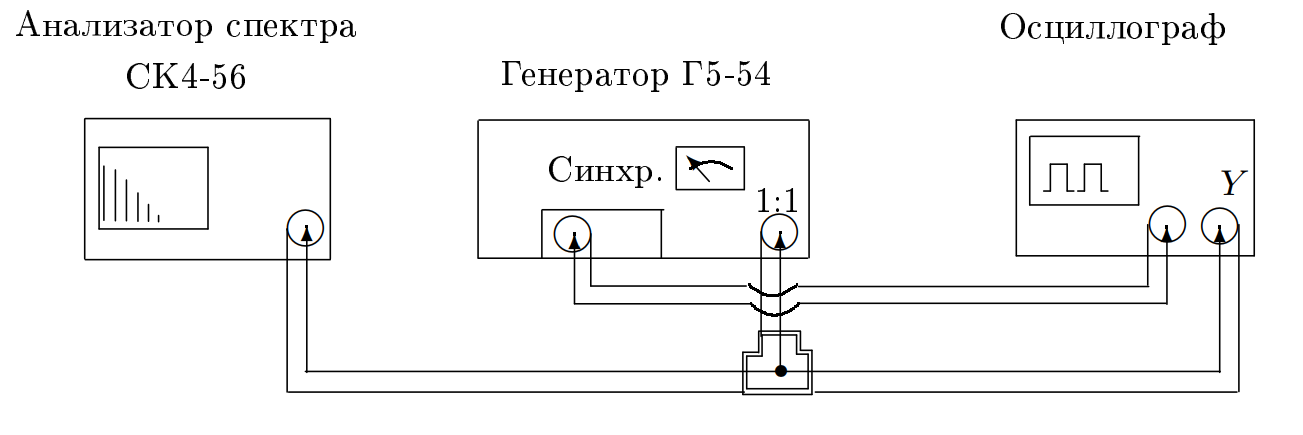
\includegraphics[width=160mm]{scheme1.png}
\caption{Схема установки для пункта А }\label{schema1.png}
\end{figure}

\textbf{Изначально на вход подавалась последовательность прямоугольных импульсов с параметрами: }

частота повторения импульсов $f_\text{повт} = 1 kHz$,

продолжительность одного импульса $\tau = 25 \mu sec$.

На рисунке \ref{A_2} видно, как меняется спектр сигнала при изменении (увеличении в два раза) каждого из этих параметров.

\begin{figure}[htpb]
\centering
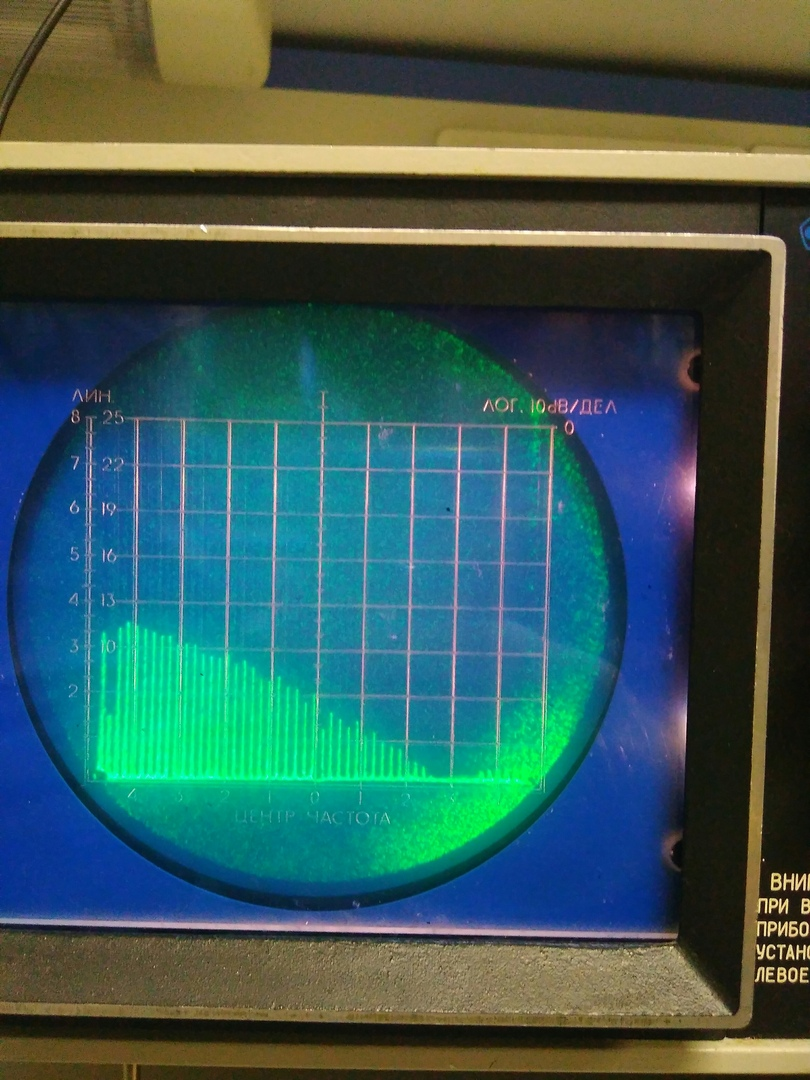
\includegraphics[width=50mm]{Pictures/A2-0.jpg}
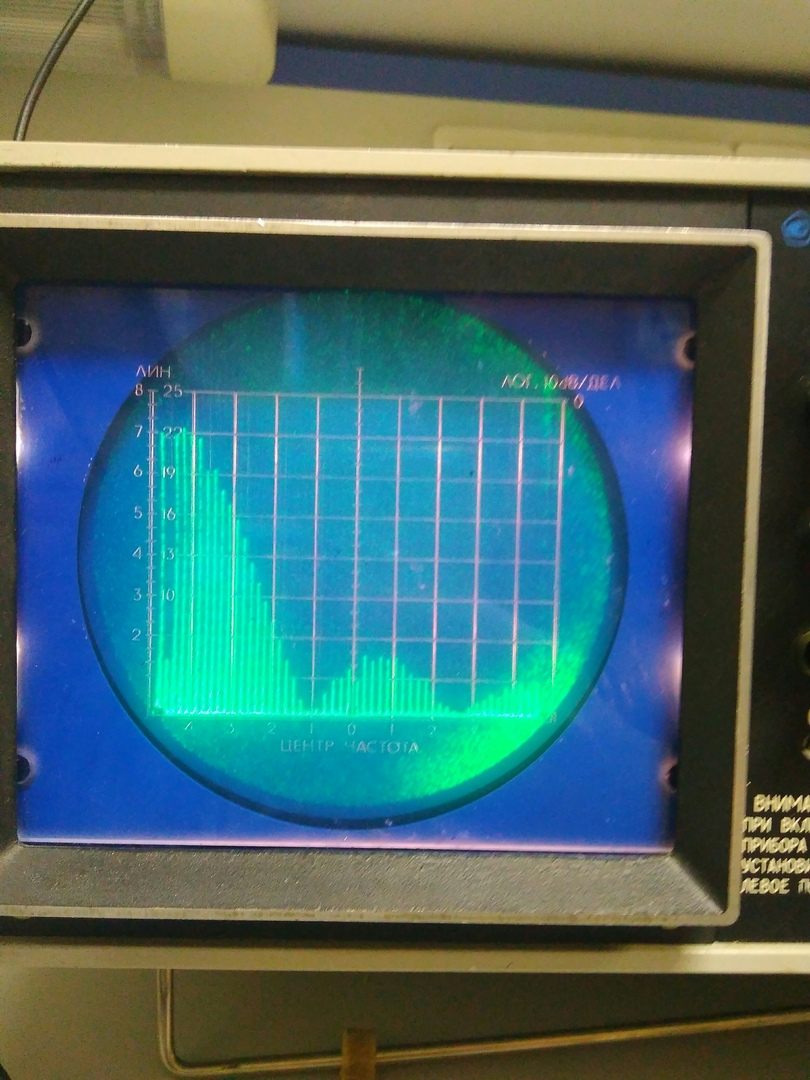
\includegraphics[width=50mm]{Pictures/A2-a.jpg}
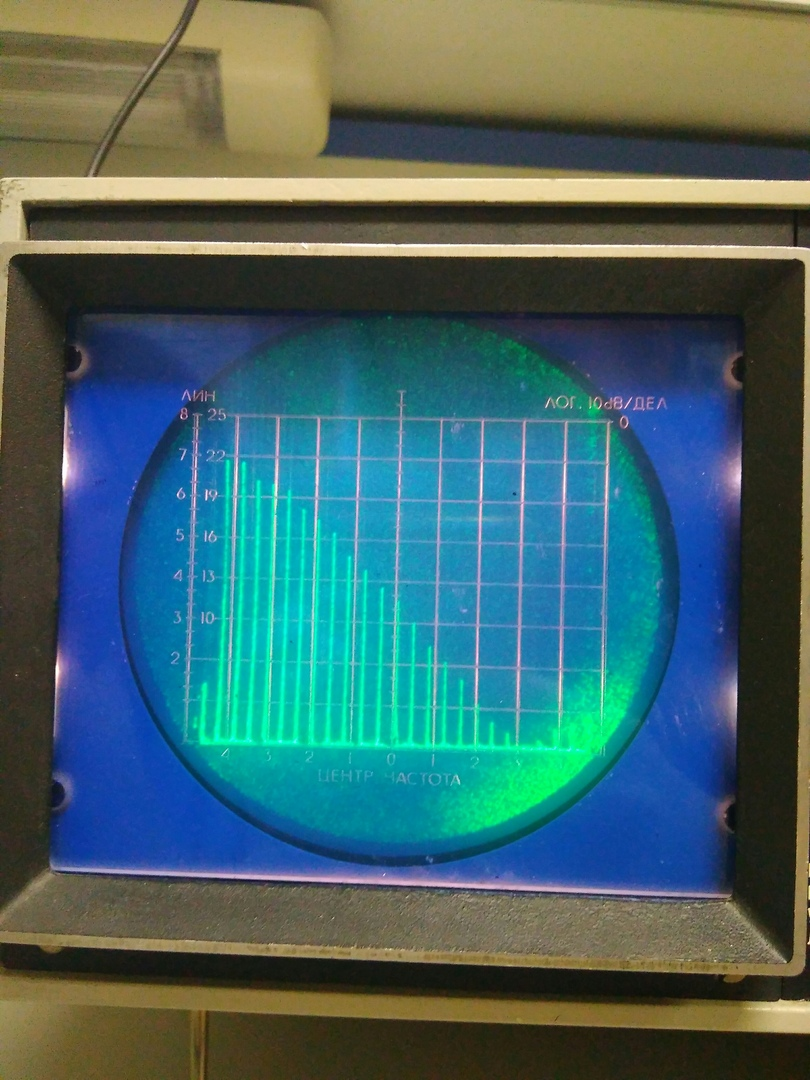
\includegraphics[width=50mm]{Pictures/A2-b.jpg}
\caption{(слева-направо) Спектр сигнала из пункта А до изменения параметров; при удвоенном $\tau$; при удвоенной $f_\text{повт}$.}
\label{A_2}
\end{figure}

Далее была получена зависимость ширины спектра $\Delta \nu$ от $\tau$ при фиксированной $f_\text{повт} = 1 kHz$ (Рис. \ref{A_5}).

\begin{figure}[tpb]
\centering
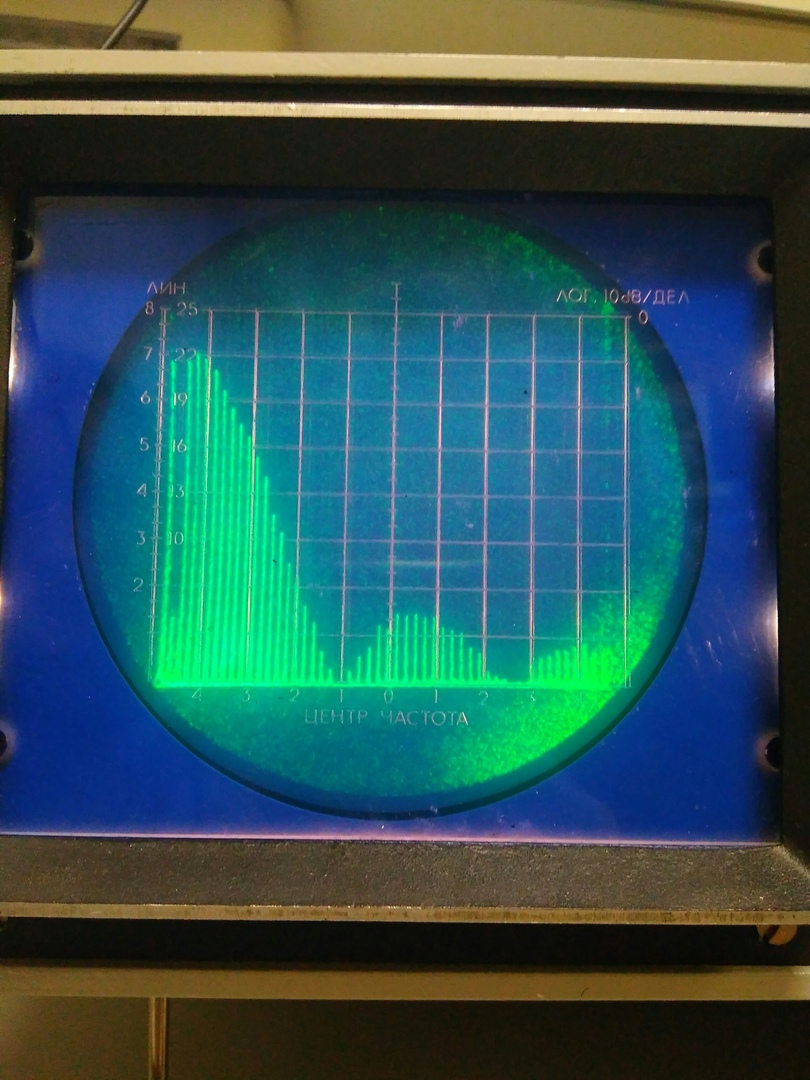
\includegraphics[width=50mm]{Pictures/A3-50.jpg}
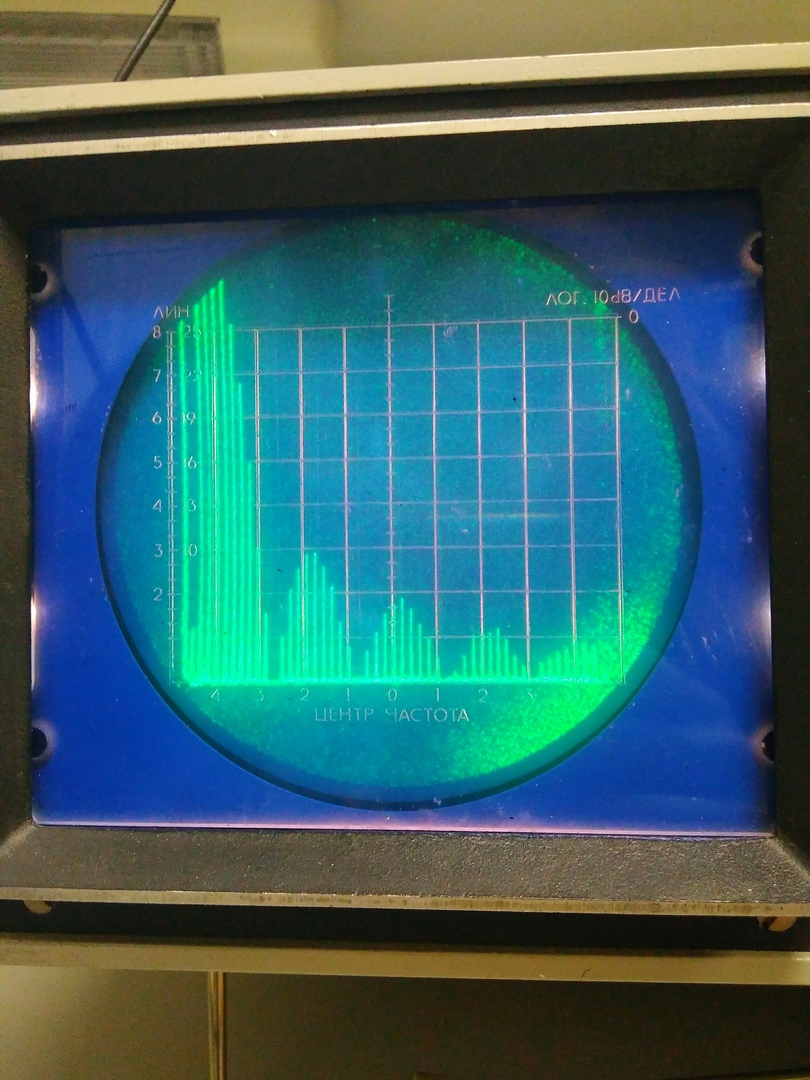
\includegraphics[width=50mm]{Pictures/A3-100.jpg}
\caption{(слева-направо) Спектры сигнала из пункта А при значениях $\tau = 50 \mu sec$ и $\tau = 100 \mu sec$.}
\label{A_4}
\end{figure}

\begin{figure}[tpb]
\centering
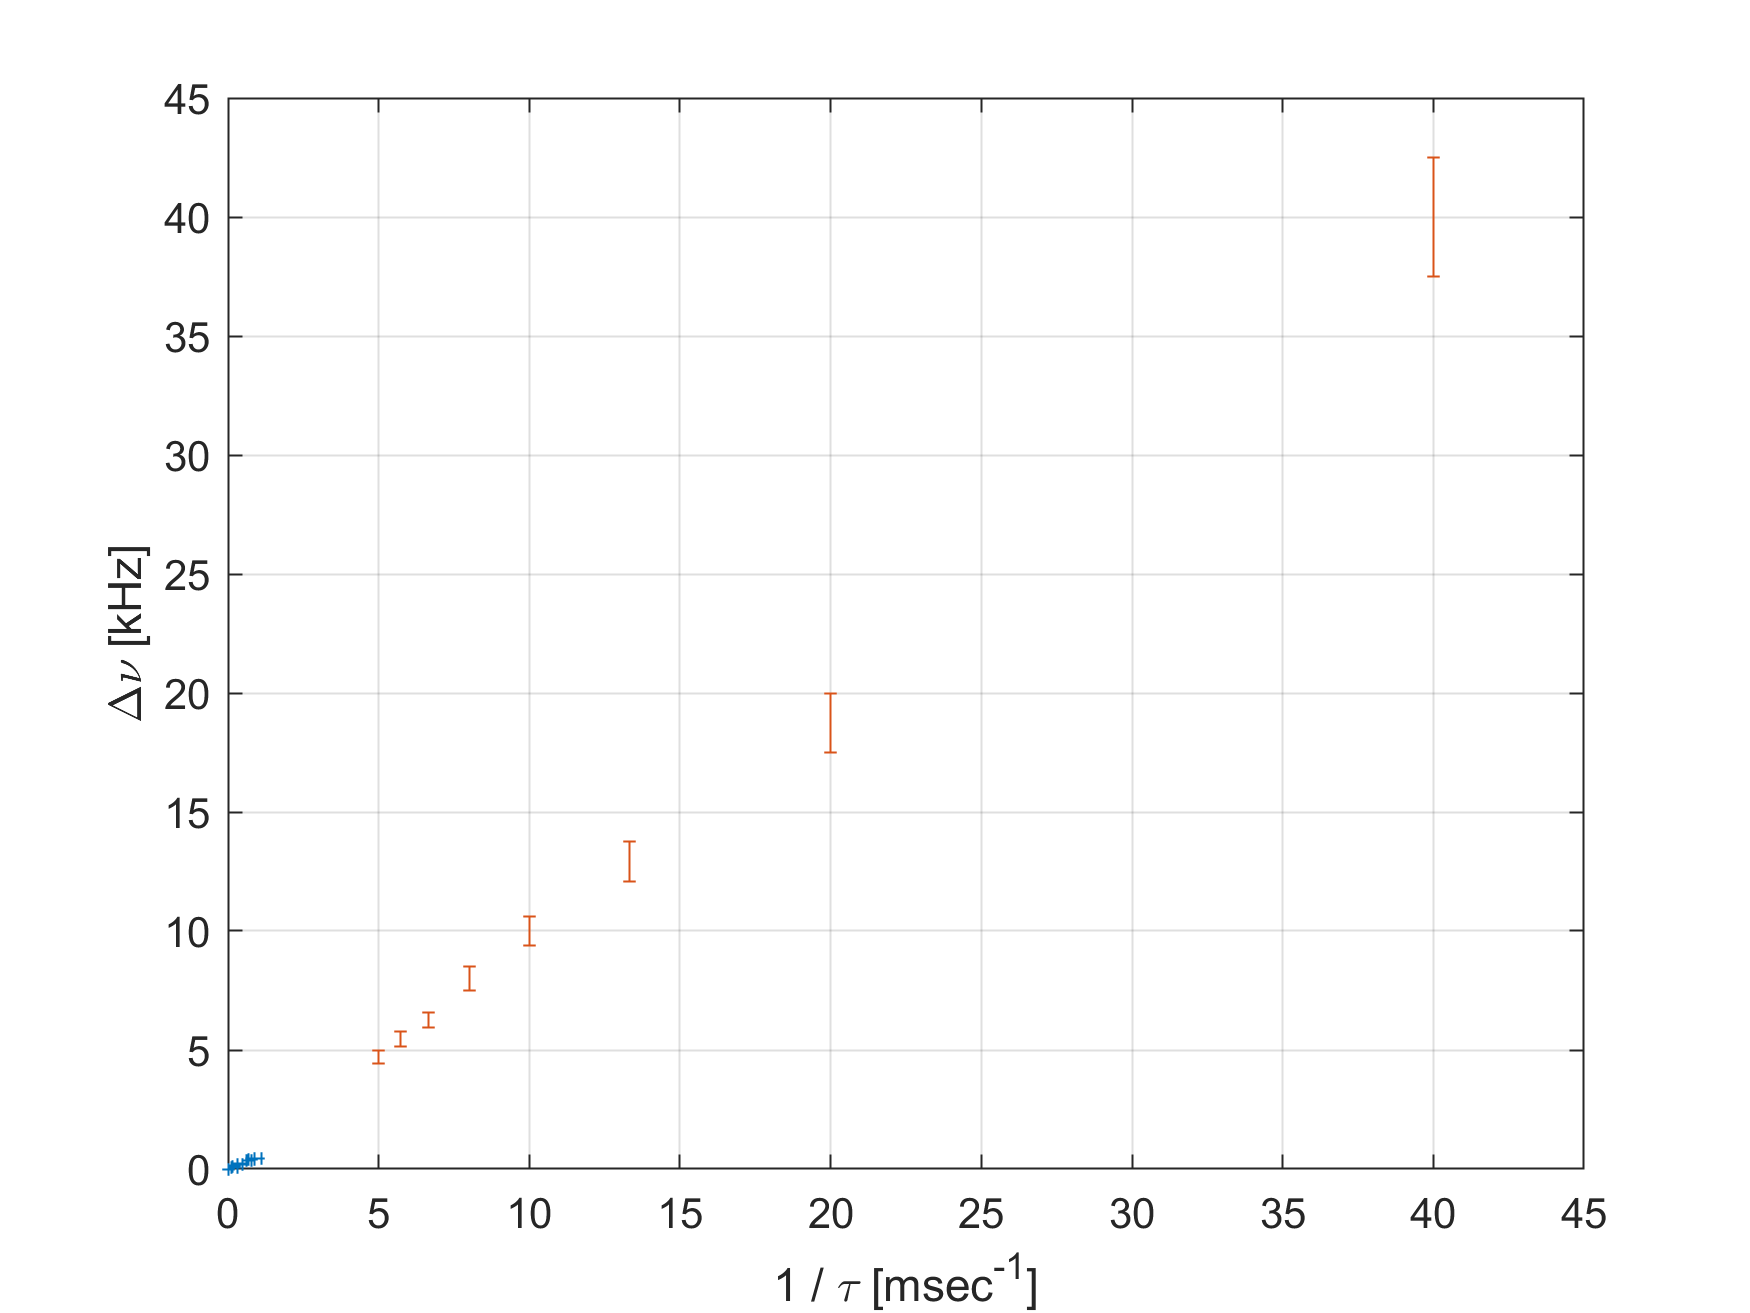
\includegraphics[width=100mm]{PlotA.png}
\caption{Зависимость ширины спектра $\Delta \nu$ от $\tau$ при фиксированной $f_\text{повт} = 1 kHz$.}
\label{A_5}
\end{figure}

Как видно, эта зависимость линейная с коэффициентом пропорциональности примерно равным единице. Что говорит о том, что $\Delta \nu \tau \approx 1$, что отвечает своего рода соотношению неопределённости: чем больше сигнал размазан по времени (чем больше $\tau$), тем точнее мы можем определить его спектр (тем меньше $\Delta \nu$).

\bigskip
\subsection*{Пункт Б}
\bigskip

\textbf{В этом пункте на вход подавалась последовательность цугов гармонических колебаний с параметрами:}

частота повторения цугов $f_\text{повт} = 1 kHz$,

продолжительность одного импульса $\tau = 50 \mu sec$,

частота несущей (гармонических колебаний) $\nu_0 = 25 kHz$.

\begin{figure}[htpb]
\centering
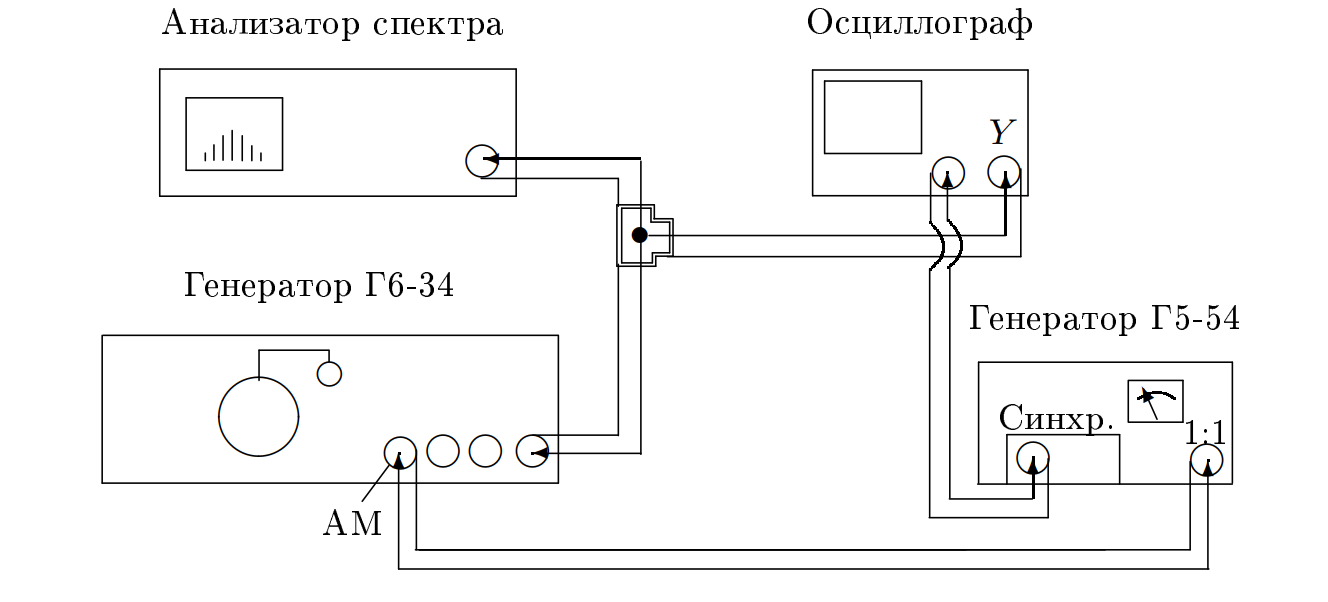
\includegraphics[width=160mm]{scheme2.png}
\caption{Схема установки для пункта Б }\label{schema}
\end{figure}

\begin{figure}[tpb]
\centering
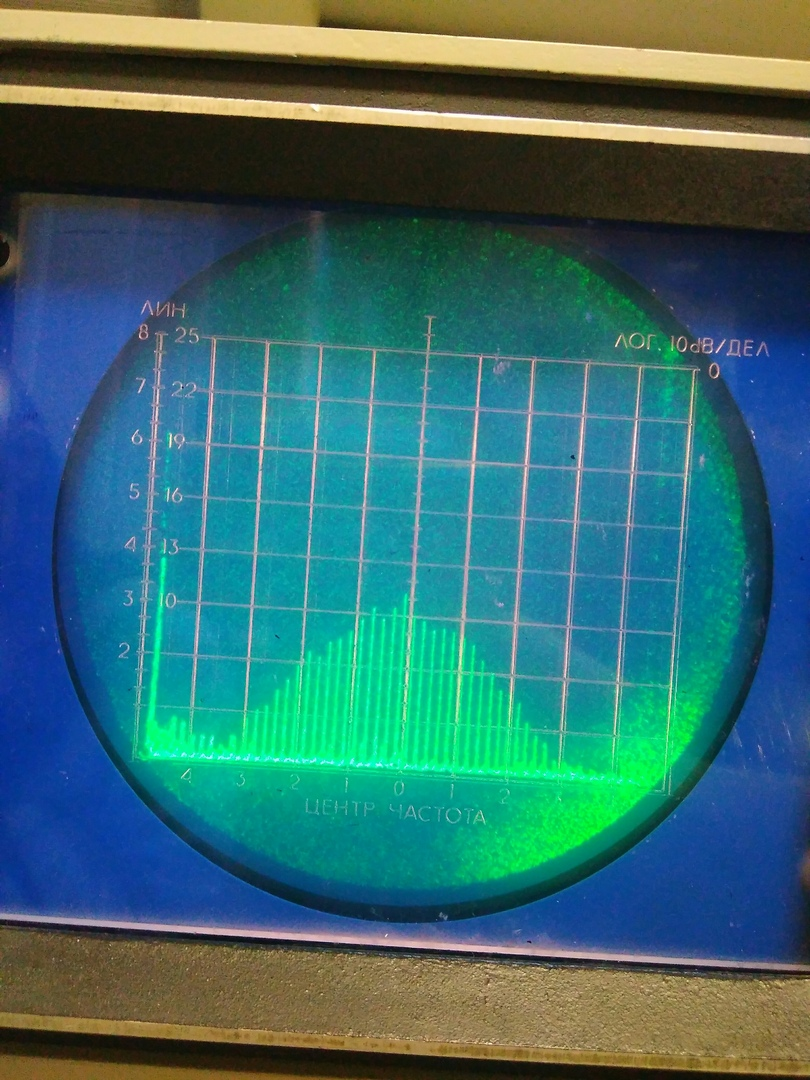
\includegraphics[width=50mm]{Pictures/B2-a50.jpg}
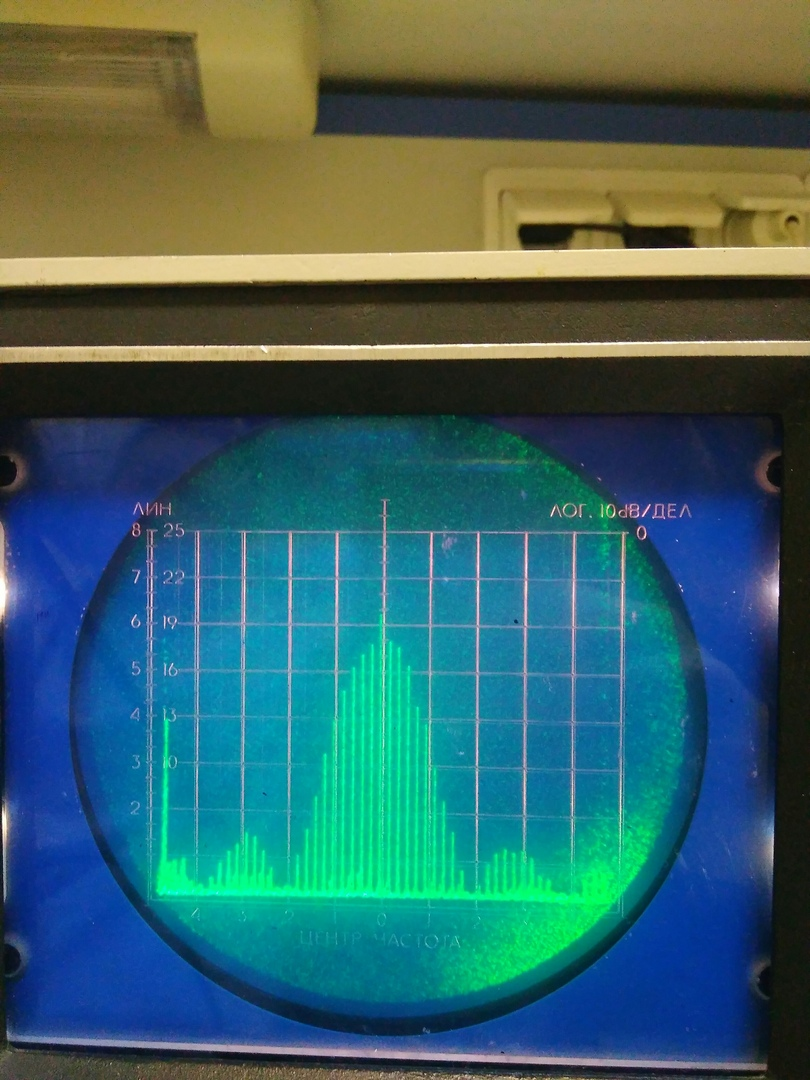
\includegraphics[width=50mm]{Pictures/B2-a100.jpg}
\caption{(слева-направо) Спектр сигнала из пункта Б до изменения параметров; при удвоенном $\tau$.}
\label{B_2a}
\end{figure}

\begin{figure}[tpb]
\centering
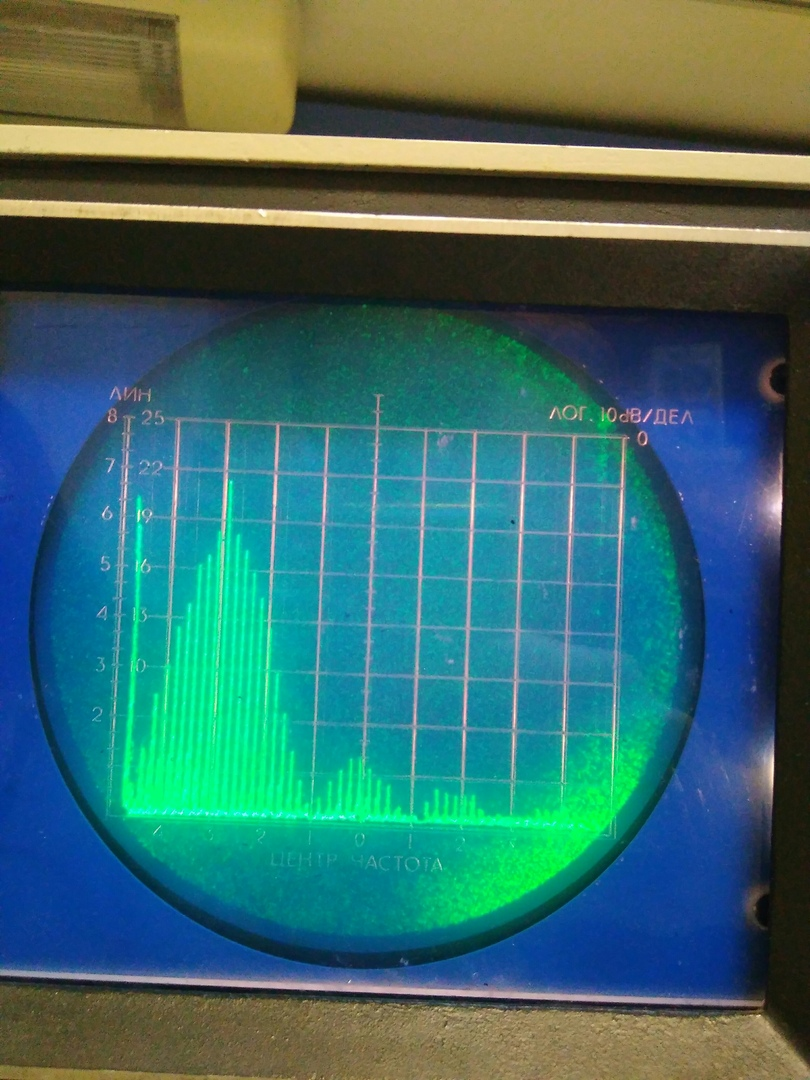
\includegraphics[width=50mm]{Pictures/B2-b10.jpg}
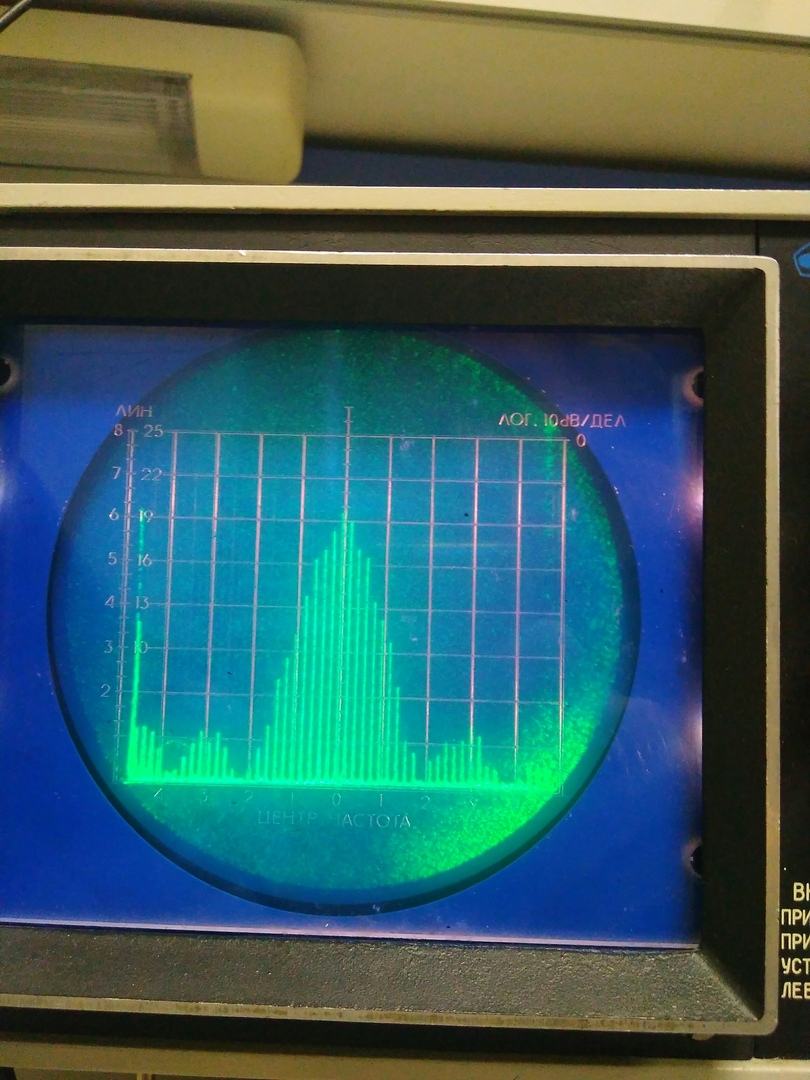
\includegraphics[width=50mm]{Pictures/B2-b25.jpg}
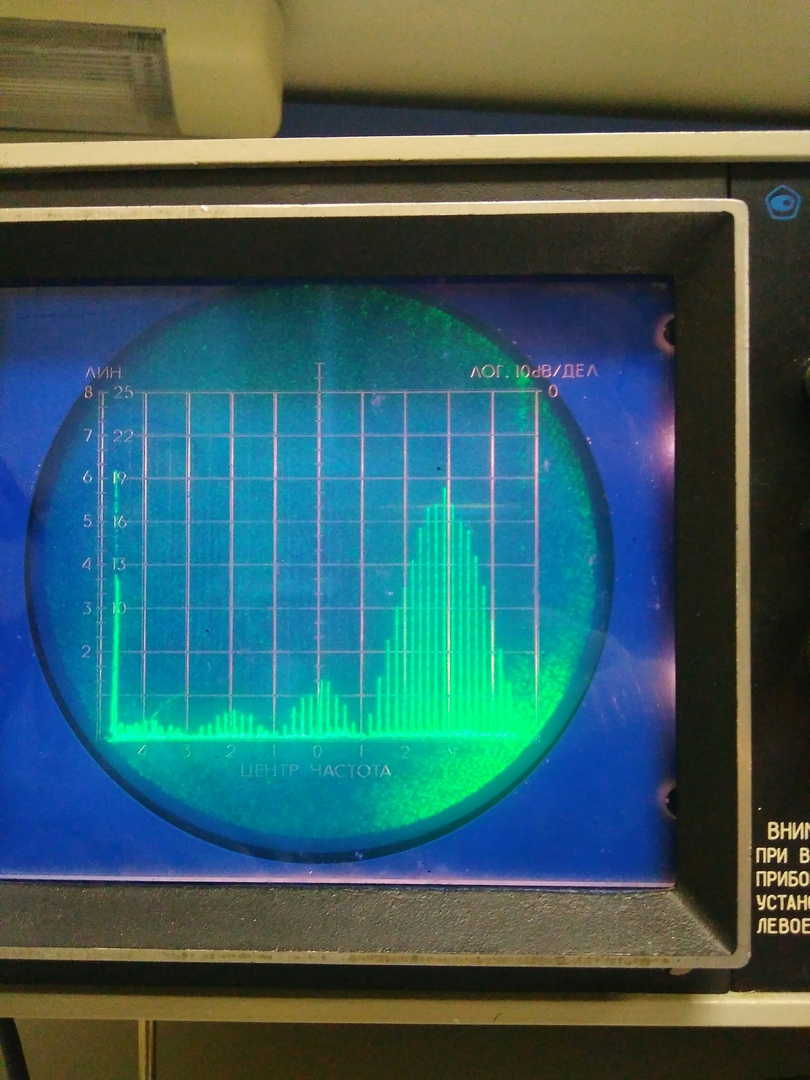
\includegraphics[width=50mm]{Pictures/B2-b40.jpg}
\caption{(слева-направо) Спектр сигнала из пункта Б при значениях несущей частоты      $\nu_0 = 10 kHz$; $\nu_0 = 25 kHz$; $\nu_0 = 40 kHz$.}
\label{B_2b}
\end{figure}

\begin{figure}[tpb]
\centering
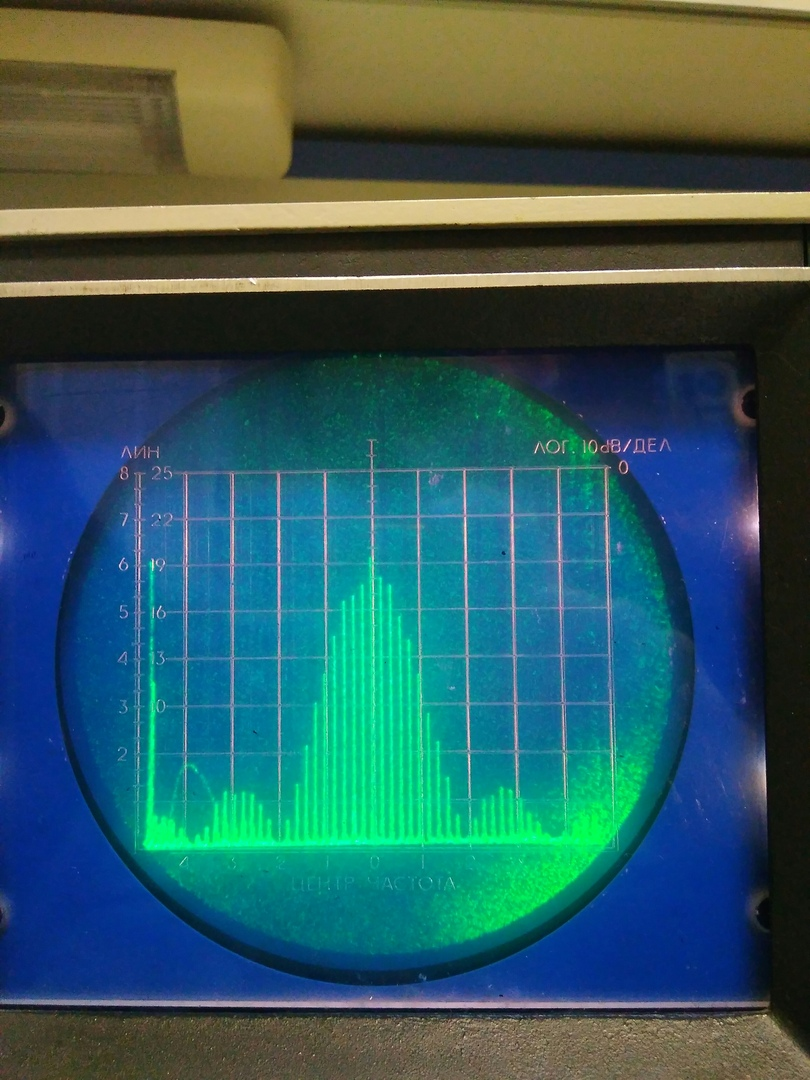
\includegraphics[width=50mm]{Pictures/B4-1.jpg}
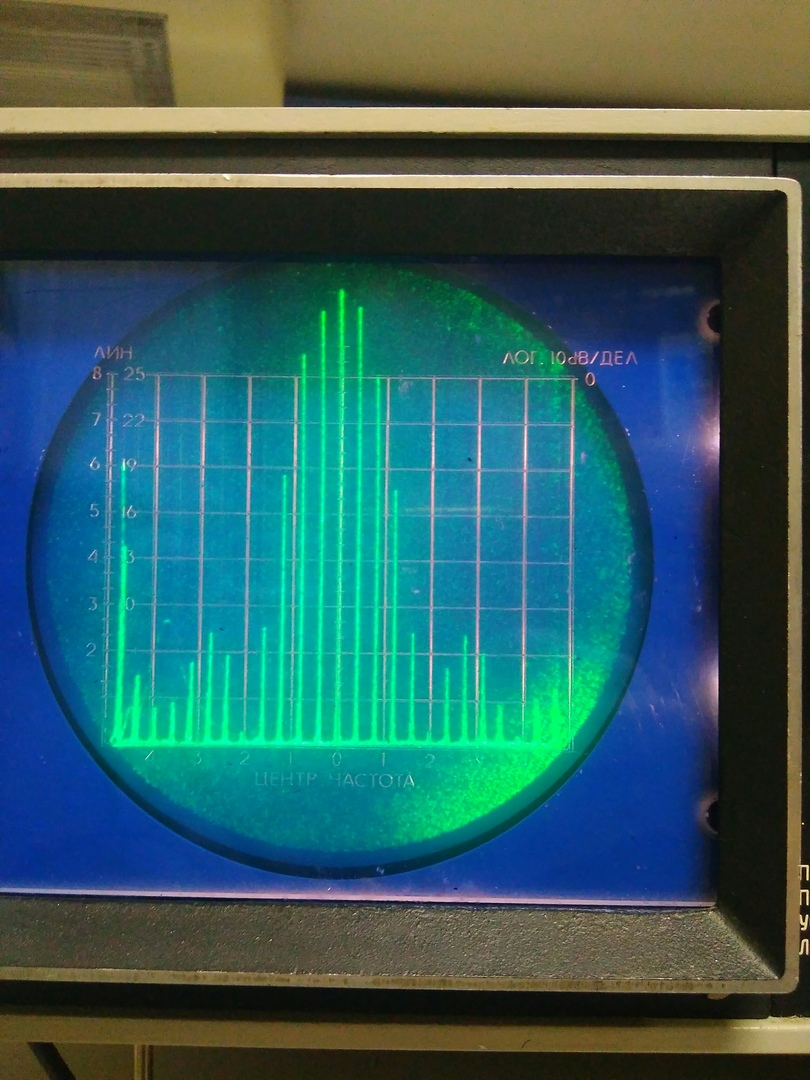
\includegraphics[width=50mm]{Pictures/B4-2.jpg}
\caption{(слева-направо) Спектр сигнала из пункта Б при $\tau = 100\mu sec$ и $f_\text{повт} = 1 kHz$; $f_\text{повт} = 2 kHz$.}
\label{B_4}
\end{figure}

На рисунках \ref{B_2a} и \ref{B_2b} видно, как изменяется спектр при изменении параметров сигнала.

Была снята зависимость расстояния между соседними спектральными линиями $\delta \nu$ от частоты повторения цугов $f_\text{повт}$. Её можно видеть на графике \ref{B_5}.

\begin{figure}[tpb]
\centering
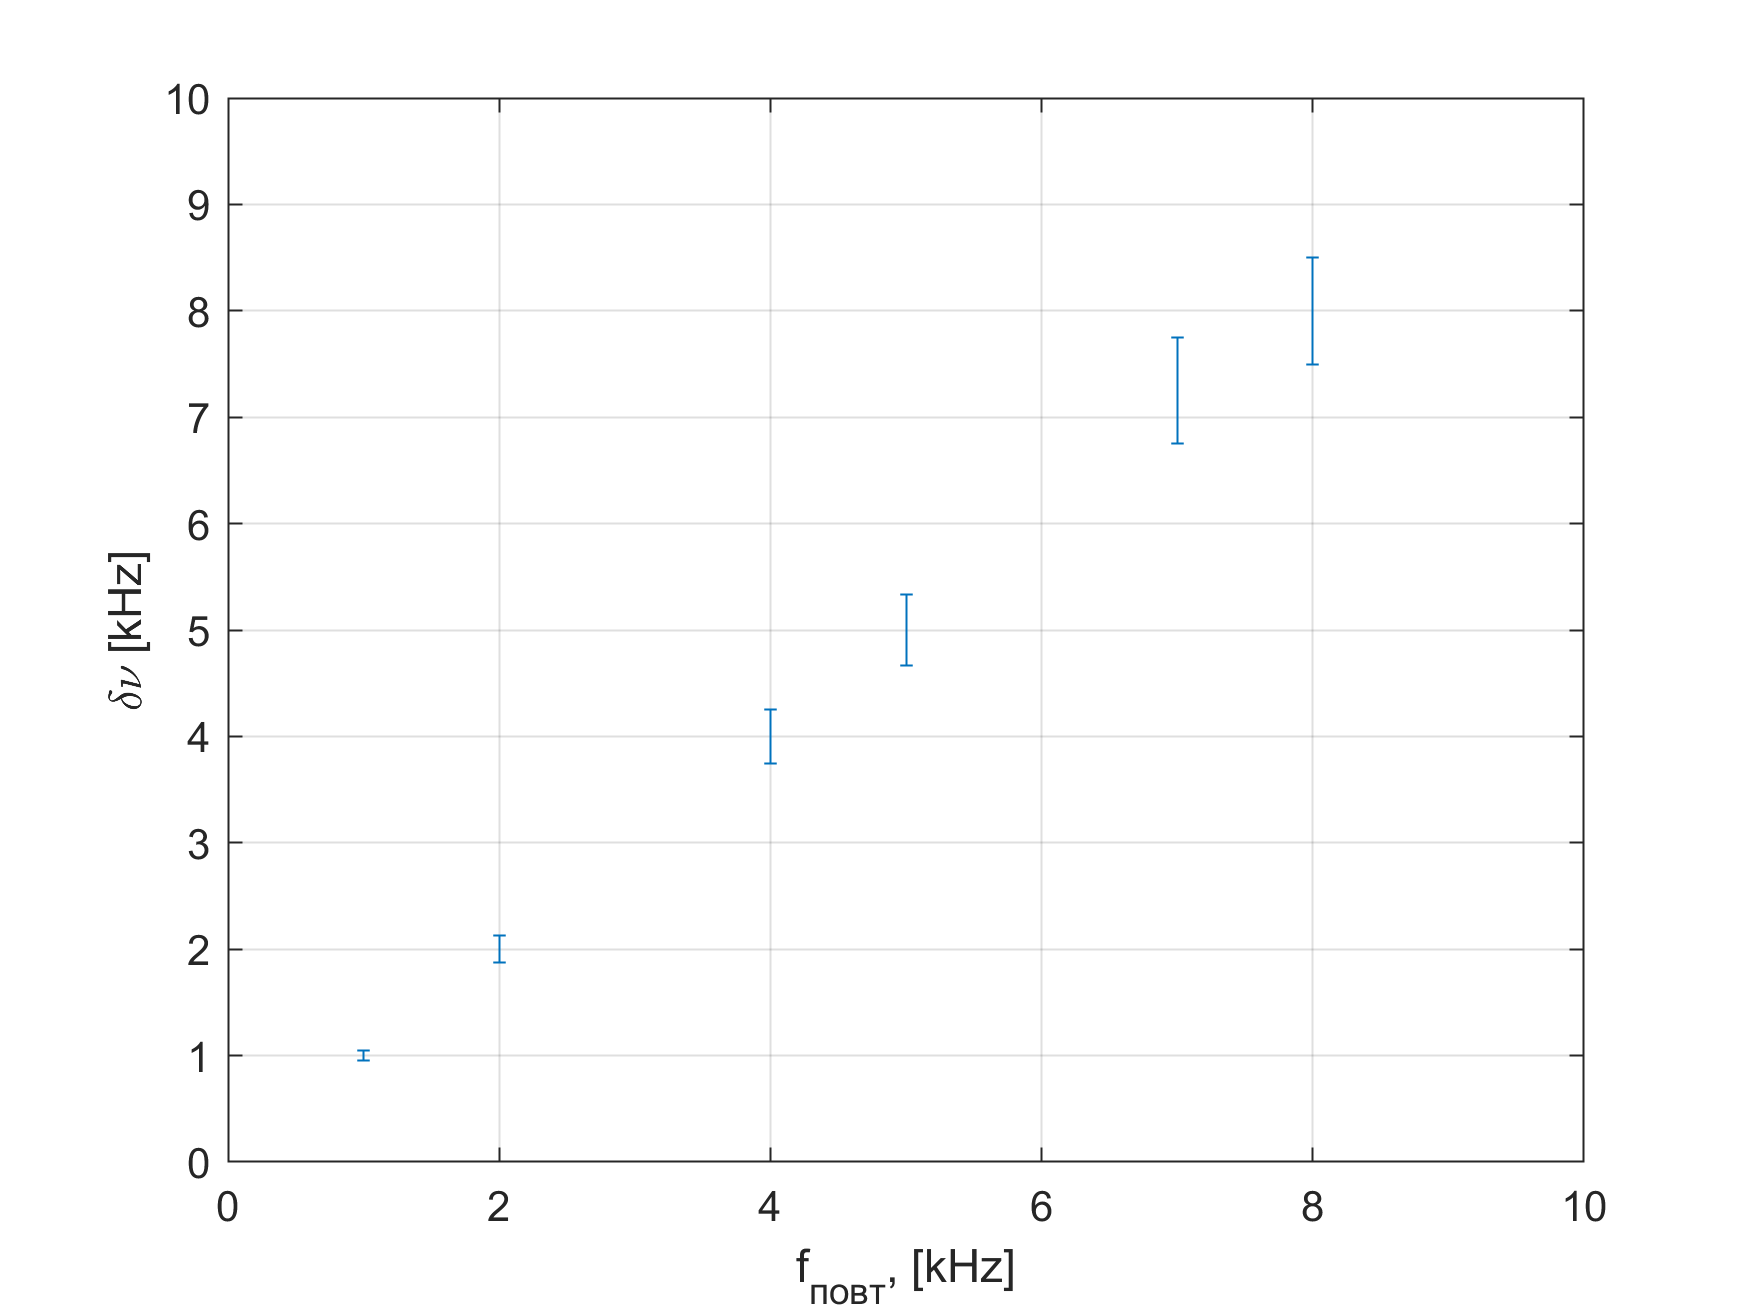
\includegraphics[width=100mm]{PlotB.png}
\caption{Зависимость расстояния между соседними спектральными линиями $\delta \nu$ от частоты повторения цугов $f_\text{повт}$}
\label{B_5}
\end{figure}

Можно видеть, что эта зависимость имеет коэффициент наклона примерно равный единице, что означает, что $\frac{\delta\nu}{f_\text{повт}} \approx 1$. Что в лабнике называют соотношением неопределённости, хотя я не до конца понимаю, где тут неопределённость (уменьшение времени между цугами (увеличение $f_\text{повт}$), т.е. уменьшение точности по времени, соответствует увеличению расстояния между соседними спектральными линиями $\delta \nu$, т.е. увеличение точности по определению $\nu_0$ ?). Но тем не менее эта штука и правда равна единице. \textbf{Я бы сказал, что это просто свойство спектрального разложения в случае дискретного спектра: линии спектра удалены друг от друга на величину частоты, определяющий периодичность всего сигнала, то-есть $f_\text{повт}$ в нашем случае.}

\bigskip
\newpage
\subsection*{Пункт В}
\bigskip

\textbf{В этом пункте на вход подавался амплитудно-моделированный сигнал с параметрами:}

частота модуляции цугов $f_\text{мод} = 1 kHz$,

частота несущей (гармонических колебаний) $\nu_0 = 25 kHz$,

и переменной глубиной модуляции $m$.

\begin{figure}[htpb]
\centering
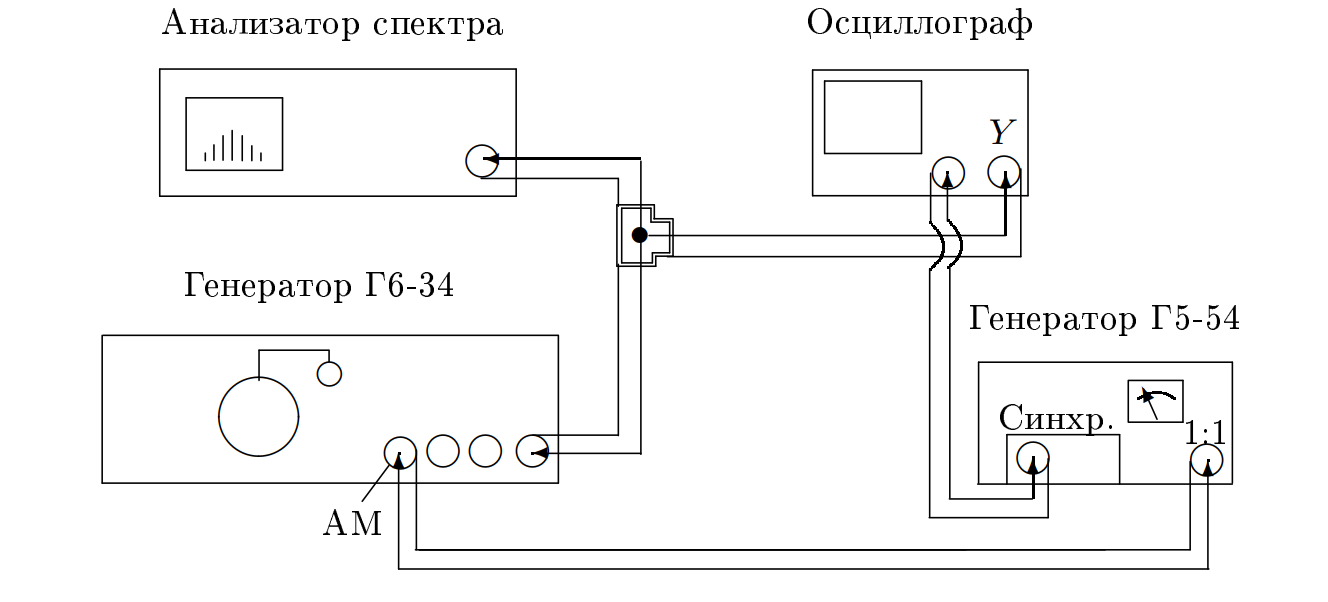
\includegraphics[width=160mm]{scheme2.png}
\caption{Схема установки для пункта В }\label{schema}
\end{figure}

\begin{figure}[htpb]
\centering
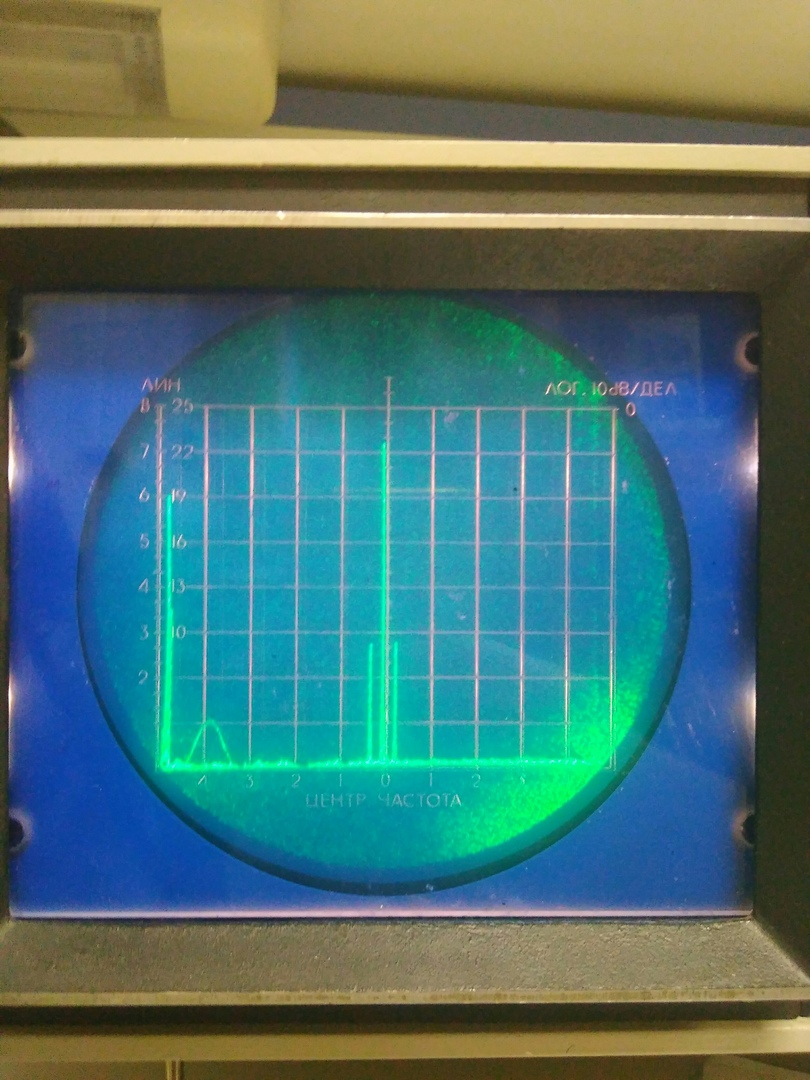
\includegraphics[width=50mm]{Pictures/C-1.jpg}
\caption{Пример спектра АМ сигнала}
\label{C}
\end{figure}

Была получена зависимость отношения амплитуды боковой линии спектра к амплитуде центральной линии $\frac{a_\text{бок}}{a_\text{осн}}$ от глубины модуляции $m$. Она представлена на графике \ref{PlotC}. Как видно, коэффициент наклона этого графика равен примерно половине, что \textbf{соответствует} значению, полученному из теории: $\frac{a_\text{бок}}{a_\text{осн}} = 0,5m$.

\begin{figure}[tpb]
\centering
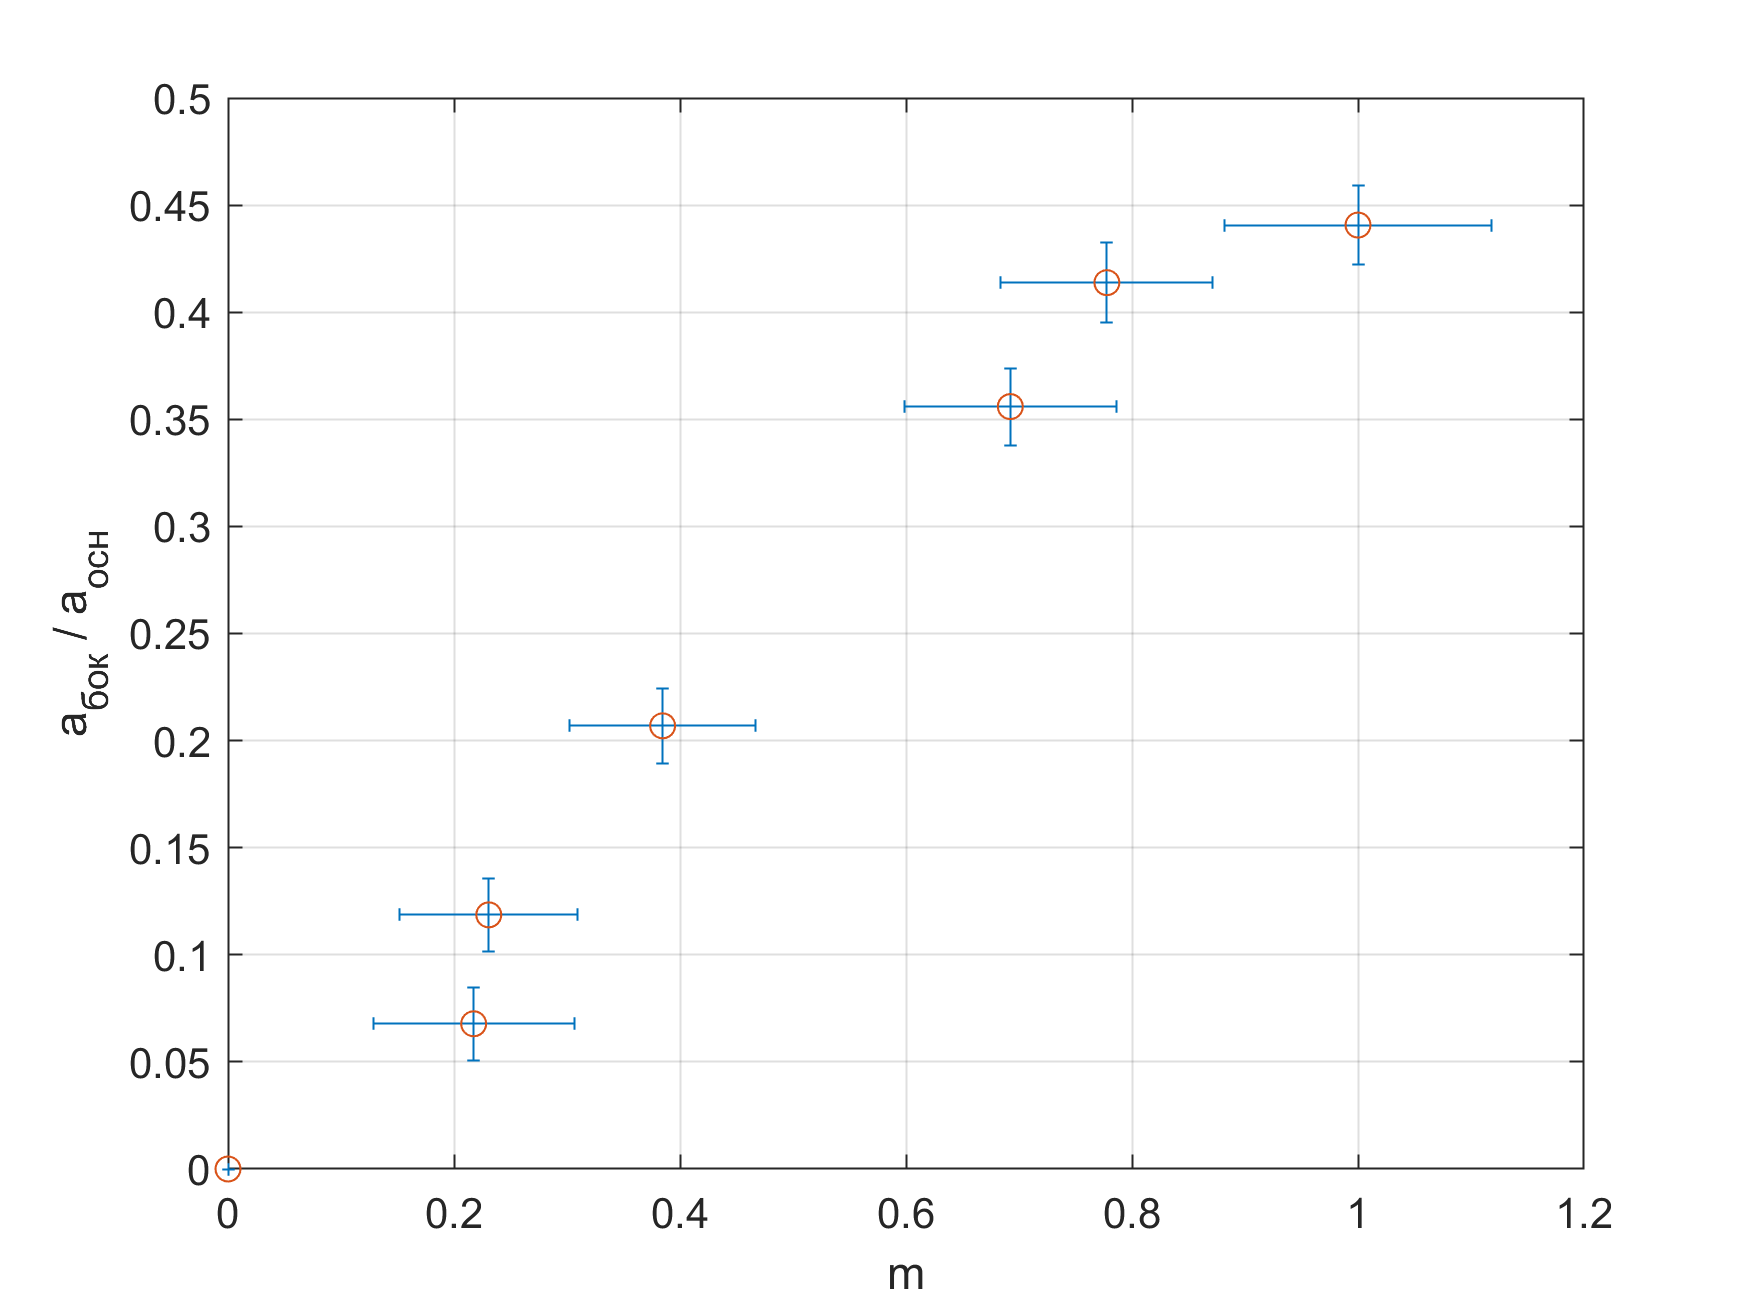
\includegraphics[width=160mm]{PlotC.png}
\caption{Зависимость отношения амплитуды боковой линии спектра к амплитуде центральной линии $\frac{a_\text{бок}}{a_\text{осн}}$ от глубины модуляции $m$.}
\label{PlotC}
\end{figure}

\bigskip


\bigskip

\subsection*{Итог}
\bigskip
\textbf{Во всех пунктах данной работы (для всех исследованных видов сигналов) предсказания из теории (соотношения неопределённости и зависимость отношения амплитуд побочных линий к амплитуде основной для спектра АМ сигнала) подтвердились на эксперименте.} Что вообще является благородным научным делом - проверять результаты, полученные другими группами. Другое дело, что эти конкретно результаты с большой вероятностью уже были проверены до меня. 
 
\subsection*{Приложение}
\bigskip

\begin{figure}[htpb]
\centering
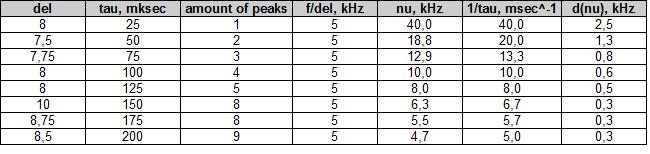
\includegraphics[width=100mm]{tableA.jpg}
\caption{Зависимость ширины спектра $\Delta \nu$ от $\tau$ при фиксированной $f_\text{повт} = 1 kHz$.}
\end{figure}

\begin{figure}[htpb]
\centering
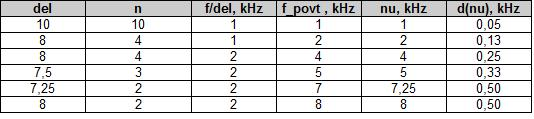
\includegraphics[width=100mm]{tableB.jpg}
\caption{Зависимость расстояния между соседними спектральными линиями $\delta \nu$ от частоты повторения цугов $f_\text{повт}$}
\end{figure}

\begin{figure}[htpb]
\centering
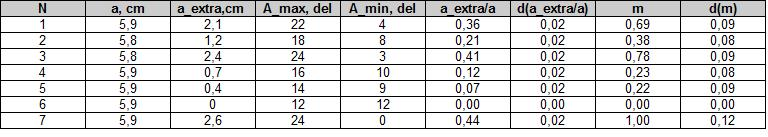
\includegraphics[width=100mm]{tableC.jpg}
\caption{Зависимость отношения амплитуды боковой линии спектра к амплитуде центральной линии $\frac{a_\text{бок}}{a_\text{осн}}$ от глубины модуляции $m$.}
\end{figure}
 
\end{document} % конец документа